\documentclass{jsarticle}
\usepackage[dvipdfmx]{graphicx}
\usepackage{listings,jlisting}
\usepackage{float}
\lstset{%
  language={C},
  basicstyle={\small\ttfamily},%
  identifierstyle={\small},%
  commentstyle={\small\itshape},%
  keywordstyle={\small\bfseries},%
  ndkeywordstyle={\small},%
  stringstyle={\small\ttfamily},
  frame={tb},
  breaklines=false,
  columns=[l]{fullflexible},%
  numbers=left,%
  xrightmargin=0zw,%
  xleftmargin=3zw,%
  numberstyle={\scriptsize},%
  stepnumber=1,
  numbersep=1zw,%
  lineskip=-0.5ex%
}

\begin{document}

\title{画像工学 レポート\\ \vspace{1cm}― 画像の高速フーリエ変換―\vspace{2cm}}
\author{IE5 (9) 片岡 駿之介 \vspace{1cm}}
\maketitle

\newpage

\section{課題}

画像処理は2次元の連続的な信号として考えることができる.そこで,この2次元の信号に対してフーリエ変換を行い,それによって得られた周波数スペクトルに対して周波数フィルタをかけることによって,画像処理を実現する方法がある.\\
今回の課題では,このフーリエ変換を高速化したFFT(Fast Fourier Transform)を用いて画像のフーリエ変換を行い,これによって得られたパワースペクトルを確認する.

\section{処理の流れ}

今回の演習では,PGMファイルを以下の手順で処理していくこととした.
\begin{enumerate}
  \item 画像を配列へ取り込む.
  \item 画像を取り込んだ配列を実部を示す配列にコピーする.同時に,虚部を表す配列を0埋めする.
  \item 実部・虚部を表す配列を引数として渡し,1行ずつfft関数を実行する.
  \item 実部・虚部を表す配列を転置する.
  \item 再び,実部・虚部を表す配列を引数として渡し,1行ずつfft関数を実行する.
  \item 実部・虚部を表す配列を転置する.
  \item 各ピクセルごとに,実部と虚部をそれぞれ2乗して足し合わせ,ルートを取ったものを出力する.
  \item 出力によって得られたデータをdatファイルに保存し,gnuplotで確認する.
\end{enumerate}

\newpage

\section{ソースリスト}

\begin{lstlisting}[caption=filter.c,label=ほげ]
  #include <stdio.h>
  #include <stdlib.h>
  #include <ctype.h>
  #include <math.h>

  #define PI 3.14159265358979323846

  FILE *fp;

  int width;
  int height;
  int max_value;

  int status;
  char buffer[128];

  static void make_sintbl(int n, double sintbl[])
  {
      int i, n2, n4, n8;
      double c, s, dc, ds, t;

      n2 = n / 2;  n4 = n / 4;  n8 = n / 8;
      t = sin(M_PI / n);
      dc = 2 * t * t;  ds = sqrt(dc * ( 2 - dc));
      t = 2 * dc;  c = sintbl[n4] = 1;  s = sintbl[0] = 0;
      for (i = 1; i < n8; i++) {
          c -= dc;  dc += t * c;
          s += ds;  ds -= t * s;
          sintbl[i] = s;  sintbl[n4 - i] = c;
      }
      if (n8 != 0) sintbl[n8] = sqrt(0.5);
      for (i = 0; i < n4; i++)
          sintbl[n2 - i] = sintbl[i];
      for (i = 0; i < n2 + n4; i++)
          sintbl[i + n2] = - sintbl[i];
  }

  static void make_bitrev(int n, int bitrev[])
  {
      int i, j, k, n2;

      n2 = n / 2;  i = j = 0;
      for ( ; ; ) {
          bitrev[i] = j;
          if (++i >= n) break;
          k = n2;
          while (k <= j) {  j -= k;  k /= 2;  }
          j += k;
      }
  }

  int fft(int n, double x[], double y[])
  {
      static int      last_n = 0;                /* 前回呼出し時の n */
      static int     *bitrev = NULL;             /* ビット反転表     */
      static double  *sintbl = NULL;             /* 三角関数表       */
      int    i, j, k, ik, h, d, k2, n4, inverse;
      double t, s, c, dx, dy;

                                                 /* 準備 */
      if (n < 0) {
          n = -n;  inverse = 1;                  /* 逆変換 */
      } else inverse = 0;
      n4 = n / 4;
      if (n != last_n || n == 0) {
          last_n = n;
          if (sintbl != NULL) free(sintbl);
          if (bitrev != NULL) free(bitrev);
          if (n == 0) return 0;                  /* 記憶領域を解放 */
          sintbl = malloc((n + n4) * sizeof(double));
          bitrev = malloc(n * sizeof(int));
          if (sintbl == NULL || bitrev == NULL) {
              fprintf(stderr, "memory error\n"); return 1;
          }
          make_sintbl(n, sintbl);
          make_bitrev(n, bitrev);
      }
      for (i = 0; i < n; i++) {                  /* ビット反転 */
          j = bitrev[i];
          if (i < j) {
              t = x[i];  x[i] = x[j];  x[j] = t;
              t = y[i];  y[i] = y[j];  y[j] = t;
          }
      }
      for (k = 1; k < n; k = k2) {               /* 変換 */
          h = 0;  k2 = k + k;  d = n / k2;
          for (j = 0; j < k; j++) {
              c = sintbl[h + n4];
              if (inverse) s = - sintbl[h];
              else         s =   sintbl[h];
              for (i = j; i < n; i += k2) {
                  ik = i + k;
                  dx = s * y[ik] + c * x[ik];
                  dy = c * y[ik] - s * x[ik];
                  x[ik] = x[i] - dx;  x[i] += dx;
                  y[ik] = y[i] - dy;  y[i] += dy;
              }
              h += d;
          }
      }
      if (! inverse)                             /* 逆変換でないなら n で割る */
          for (i = 0; i < n; i++) {  x[i] /= n;  y[i] /= n;  }
      return 0;                                                /* 正常終了 */
  }


  void image_open(char *file_name) {
    if ((fp = fopen(file_name, "r")) == NULL) {
  		printf("file open error!!\n");
  		exit(-1);	/* (3)エラーの場合は通常、異常終了する */
  	}
    // printf("%s\n", file_name);
  }

  int main(int argc,char *argv[]) {

    /* 入力コマンドのチェック */
    if(argc == 1) {
      printf("Usage : ./fft <pgm file name>\n");
      exit(0);
    } else if (argc == 2) {
      image_open(argv[1]);
    }

    /* ヘッダ取得部 */
    int ch;

    while (status < 3) {
      ch = getc(fp);

      if(ch == '#') { // コメントのスキップ
        while (( ch = getc(fp)) != '\n')
          break;
      }

      if(ch == 'P') { // マジックナンバーのチェック
        if(getc(fp) != '5') {
          printf("Magic Number is wrong.\n");
          break;
        } else {
          // printf("Magic Number is P5\n");
        }
      }

      if(isdigit((unsigned char)ch)) { // 数値取得部
        buffer[0] = ch;
        int i=1;
        while(1) {
            char c = getc(fp);
            if(isdigit((unsigned char)c)) {
              buffer[i]=c;
              i++;
            } else
              break;
        }
        buffer[i] = '\0';

        switch (status) {
          case 0: // width取得部
            width = atoi(buffer);
            // printf("width=%d\n", width);
            break;
          case 1: // height取得部
            height = atoi(buffer);
            // printf("height=%d\n", height);
            break;
          case 2: // max_value取得部
            max_value = atoi(buffer);
            // printf("max_value=%d\n", max_value);
            break;
        }
        status++; // 次のステータスへ
      }
    }

    /* 画素値取得部 */
    int image[width][height];

    for(int i = 0; i < height; i++) {
      for(int j = 0; j < width; j++) {
        image[j][i] = (int)getc(fp);
      }
    }

    double x[width][height];
    double y[width][height];

    for(int i = 0; i < height; i++) {
      for(int j = 0; j < width; j++) {
        x[j][i] = (double)image[j][i];
        y[j][i] = 0.0;
      }
    }

    for(int i = 0; i < height; i++) { //1かいめのfft
        fft(256, x[i], y[i]);
    }

    double x_tmp[width][height];
    double y_tmp[width][height];

    for(int i = 0; i < height; i++) { //1かいめの転置
      for(int j = 0; j < width; j++) {
        x_tmp[i][j] = x[j][i];
        y_tmp[i][j] = y[j][i];
      }
    }

    for(int i = 0; i < height; i++) {
      for(int j = 0; j < width; j++) {
        x[i][j] = x_tmp[i][j];
        y[i][j] = y_tmp[i][j];
      }
    }

    for(int i = 0; i < height; i++) { //2かいめのfft
        fft(256, x[i], y[i]);
    }

    for(int i = 0; i < height; i++) { //2かいめの転置
      for(int j = 0; j < width; j++) {
        x_tmp[i][j] = x[j][i];
        y_tmp[i][j] = y[j][i];
      }
    }

    for(int i = 0; i < height; i++) {
      for(int j = 0; j < width; j++) {
        x[i][j] = x_tmp[i][j];
        y[i][j] = y_tmp[i][j];
      }
    }

    for(int i = 0; i < height; i++) { //出力
      for(int j = 0; j < width; j++) {
        printf("%d %d %f\n", i, j, sqrt(pow(x[j][i], 2) + pow(y[j][i], 2)));
      }
      printf("\n");
    }

  }


\end{lstlisting}

\newpage

\section{結果}
結果の確認には,配布された「cup.pgm」を用いた.
\begin{figure}[H]
  \begin{center}
    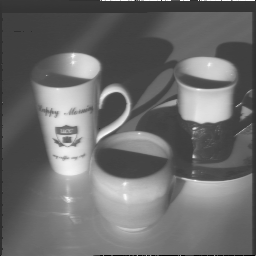
\includegraphics[width=5cm]{cup.png}
    \caption{cup.pgm}
  \end{center}
  \label{}
\end{figure}

以下に,FFTを行った際のパワースペクトルグラフを示す.

\begin{figure}[H]
  \begin{center}
    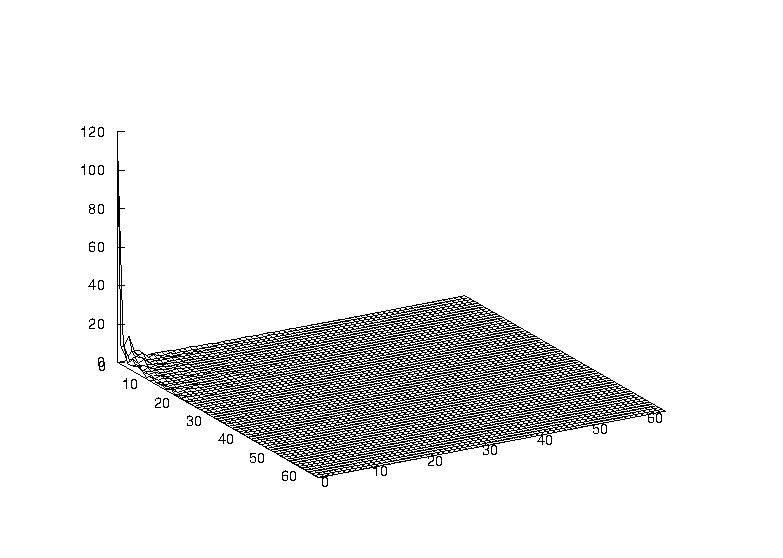
\includegraphics{../power.eps}
    \caption{cup.pgmに対してFFTを行った際のパワースペクトル}
  \end{center}
  \label{}
\end{figure}

\newpage


\section{考察}

画像をフーリエ変換した際の周波数スペクトルは,低周波数成分に集中していることがわかった.\\今まではピクセル操作で画像処理を行っていたが,周波数フィルタをかけるともっと簡単に実装できそうであると感じた.

\section{感想}
FFTが本当に高速で感動した.

\end{document}
